\chapter{Hintergrund}

\label{cha:background}
\textit{In diesem Kapitel werden die genutzten Technologien erläutert}

\section{Containervirtualisierung}

Containervisualisierung (auch Containerisierung genannt) beschreibt das Bereitstellen einer Applikation, indem die Applikation und alles, was diese zum Laufen benötigt ((System-)Bibliotheken, ausführbare Dateien, (System-)Konfigurationen, etc.) in Form eines Container-Images bereitgestellt wird. Das ermöglicht es, die Applikation isoliert, schnell und zuverlässig auf unterschiedlichen Host-Systemen auszuführen.

Im Gegensatz zur klassischen Virtualisierung wird nicht die Hardware-Ebene abstrahiert und ein komplett eigenständiges Betriebssystem hochgefahren, sondern lediglich die Betriebssystem-Ebene abstrahiert.

Das hat zur Folge, dass Containervirtualisierung weniger Speicher verbraucht und performanter im Vergleich zu Hardwarevirtualisierung ist.

\section{OCI-Container-Image Spezifikation}

Die Open Container Initiative (OCI) ist eine Organisation, welche sich auf die Standardisierung von Containern spezialisiert hat. Mitglieder dieser Initiative sind u.A. Microsoft, Amazon Web Services, Google und Red Hat. Die von OCI bereitgestellte Spezifikation definiert den aufbau eines Container-Images.

\section{ContainerD}

ContainerD ist ein System-Daemon, welcher die OCI-Image-Spezifikation unterstützt und die Verwaltung Containern übernimmt. Docker nutzt ContainerD als Backend für die Containervisualisierung. Das Unternehmen hinter Docker hat ContainerD als Open-Source-Projekt veröffentlicht und arbeitet an diesem.

\begin{figure}[H]
    \includegraphicsWeb[width=\linewidth]{https://containerd.io/img/architecture.png}
    \captionof{figure}{ContainerD Architektur: https://containerd.io/img/architecture.png}
\end{figure}


ContainerD selber ist in mehrere Komponenten aufgeteilt. Diese beinhalten unter anderem:

Eine API um mit unterschiedlichen ContainerD-Clients (Frontends) zu kommunizieren. Hierzu zählen CRI und die native ContainerD-Schnittstelle. CRI ist selber nur ein Wrapper um die native ContainerD-Schnittstelle. Die CRI-Schnittstelle wird größtenteils von Kubernetes genutzt, um ContainerD zu steuern. Die native ContainerD-Schnittstelle wird unter anderem von Docker genutzt.

Der ContainerD-Core, welcher alle nötigen Metadaten und Funktionalitäten bereitstellt, um Container zu verwalten. Dieser kommuniziert wiederrum mit dem ContainerD-Backend.

Das ContainerD-Backend ist wiederrum für die eigentliche Ausführung der Container zuständig. Es abstrahiert die dafür nötigen OS-Funktionalitäten für den ContainerD-Core. Diese Abstraktionen müssen durch einen sogenannten "Shim" implementiert werden. Der Shim ist ein kleines, plattformspezifisches Programm. Runc und d-shim sind Beispiele für Shims, welche auf Linux laufen. Runhcs wiederrum ist ein Shim, welches auf Windows läuft und Windows-Container unterstützt.  

ContainerD benötigt erweiterte rechte auf dem Host-System. Aus diesem Grund läuft ContainerD standardmäßig als Root-Prozess. Es ist mlglich diesen ohne Root-Rechte zu verwenden, allerdings nur mit einem deutlichen Mehraufwand.

\section{Docker}

Docker ist eine der bekanntesten Containervisualisierungs-Lösungen. Sie beinhaltet eine Reihe von Werkzeugen zum Erstellen, verwalten und ausführen von Containern. Docker ist ein Frontend für ContainerD.

\subsection{Dockerfile}

Eine Dockerfile ist die Definition, welche Docker benötigt, um ein Container-Image zu erstellen . In ihr werden alle nötigen Schritte sowie Metainformation definiert, um einen Container mit einer lauffähigen Applikation zu haben. Die in der Dockerfile definierten Schritte werden isoliert auf einem Basis-Image ausgeführt. Das durch die Dockerfile erstelle Image ist somit das Resultat alle Schritte, aus dem das Basis-Image entsteht und den in der Dockerfile definierten Schritten \cite{dockerDockerfileOverview}.

Hier ist ein simples Dockerfile Beispiel für das Erstellen eines Julea Container-Images:

\inputminted{docker}{./code-examples/Dockerfile.example}

\subsection{OCI-Container-Image Layer}

Ein OCI-Container-Image setzt sich aus Schichten (Layer) zusammen, welche stapelweise angeordnet sind. In jeder Schicht werden Änderungen an der vorherigen Schicht vorgenommen. Jedes OCI-Container-Image hat ein sogenanntes "Base-Image". Dieses ist die erste Schicht. Ein "Base-Image" ist üblicherweise ein spezifisches Betriebssystem (z. B.: Debian, Ubuntu, Windows, etc.).

\subsection{Docker Build-Cache}

Docker verfügt über Caching-Mechanismen, welche subsequente Builds beschleunigen \cite{dockerCache}. Das Caching funktioniert, indem Docker jedes einzelne "Layer" zwischenspeichert. Wenn sich ein Layer ändert, müssen nur die Layer, welche direkt oder indirekt auf dem Layer aufbauen, neu ausgeführt werden. Um das caching möglichst effektiv zu verwenden, sollte man also sicherstellen, dass Layer, welche besonders lange zum Erstellen brauchen, möglichst nur dann neu erstellt werden, wenn dies auch notwendig ist.

\subsection{Docker BuildKit}

Docker BuildKit ist das neue Backend um OCI-Container-Images mit Docker zu erstellen. Ziel von BuildKit ist es, den Docker Legacy Builder zu ersetzen \cite{dockerBuildKit}.

Docker BuildKit hat viele Verbesserungen, um Docker Builds, im Vergleich zum Docker Legacy Builder, performanter zu machen. Dazu zählen: Parallelisierung von Build-Stages, Auslassen von unbenutzten Build-Stages, mehr Caching Möglichkeiten wie z. B. Cache-Mounts, u. v. m.

Docker BuildKit Backends müssen nicht explizit auf dem Computer installiert werden, auf dem man entwickelt. Docker kann auch BuildKit Backend von Remote-Servern einbinden. Das ermöglicht es, Builds auf leistungsstärkeren Servern, sowie auf Servern mit einer anderen CPU-Architektur auszuführen, um die Build-Zeit zu verkürzen.

\subsubsection{Docker Buildx}

Um das Docker BuildKit Backend mit Docker zu verwenden, nutzt man Docker Buildx \cite{dockerDockerBuildx}. Docker Buildx ist eine offizielle Docker Erweiterung. Docker Buildx hat einige Funktionalitäten um Docker BuildKit Backends einzubinden, sowie festzulegen welche BuildKit Backends man verwenden möchte.

\subsubsection{Docker Buildx Bake}

Eine weitere Funktionalität von Docker Buildx ist Docker Buildx Bake \cite{dockerBake}. Docker Buildx Bake ermöglicht es mithilfe einer sog. Bakefile das erstellen und mehrerer OCI-Container-Images zu vereinfachen.

Momentan wird Julea in mehreren Ubuntu-Versionen sowie mit mehreren Compilern kompiliert und getestet. Somit müssten mehrere Dockerfiles ertellt werden, um alle Kombinationen zu testen. Mit Docker Buildx Bake kann man das Erstellen mehrerer Docker-Container-Images vereinfachen.

\inputminted{./lexers/docker-bake-lexer.py}{./code-examples/docker-bake.example.hcl}

\section{Container-Images für Entwicklungsumgebungen}

Während sich die "klassische" Containerisierung darauf fokussiert eine produktive Applikation zuverlässig auszurollen, fokussieren sich die Container-Images für Entwicklungsumgebungen darauf Entwicklern eine einheitliche Container-Umgebung zum Testen und Entwickeln bereitzustellen. Im Idealfall sollte ein Entwicklungs-Container den einstieg in ein Projekt/eine Entwicklungsumgebung erleichtern, indem im Container bereits alles eingerichtet ist, um an einem Projekt effektiv zu arbeiten.

Solche Container-Images sollten alle nötigen Abhängigkeiten, welche man zum Entwickeln benötigt, enthalten. Dazu zählen z. B. Compiler, Interpreter, Bibliotheken, Tools.

Im fall von Julea muss ein solcher Entwicklungs-Container alle Abhängigkeiten enthalten, um an oder mit Julea zu entwickeln. Diese Abhängigkeiten müssen kompiliert werden. Das Kompilieren ist sehr zeitaufwendig. Darum sollte ein fertiges Container-Image diese Abhängigkeiten beinhalten, sodass das initiale Kompilieren der Abhängigkeiten übersprungen werden kann.

Ein Container-Image alleine müsste allerdings immernoch vom Entwickler selber in den Editor/IDE integriert werden, da das Denutzen des Containers sonst sehr aufwändig wär. Um die integration in den Editor/IDE zu vereinfachen, bietet Microsoft eine offene Spezifikation ("Development Container") an. Wenn ein Editor/IDE diese Spezifikation unterstützt, kann der Entwickler mit einem Klick den Container in den Editor/IDE integrieren.

Neben der einfachen Integration in den Editor/IDE ermöglicht die Spezifikation eine reihe an einstellungsmöglichkeiten. So kann der Entwickler z. B. festlegen, welche Extensions installiert werden sollen, welche Umgebungsvariablen gesetzt werden sollen, welche Ports nach außen freigegeben werden sollen, welche Editor/IDE-Einstellungen gesetzt werden sollen, u. v. m.


\subsection{Editor/IDE-Unterstützung}

\begin{table}[H]
    \begin{NiceTabular}{X|X|X[4]}[hlines]
        IDE/Editor Name    & Unterstützung & Anmerkung \\
        Visual Studio Code & Ja            & Vollständige Unterstützung                                                                                                                                                                                              \\
        CLI                & Ja            & Es existiert ein offizielles CLI in form eines NPM-Paketes @devcontainer/cli. Dadurch ist es auch möglich \(Neo-\)VIM und andere Terminal-Texteditoren mit Devcontainern zu verwenden                                   \\
        Visual Studio      & Ja*           & Stand 01.12.2024: Eigeschränkte unterstützung. Aktuell sind nur C++-Projekte mit CMake unterstützt                                                                                                                      \\
        JetBrains IDEs     & Ja*           & Stand 01.12.2024 ist die unterstützung in der Beta-Phase und unvollständig.                                                                                                                                             \\
        VIM                & Ja*           & Stand 01.12.2024 gibt es ein community plugin für Neo-VIM welches devcontainer integration ermöglicht. Die vollständigkeit dieses Plugins wurde nicht überprüft. Siehe: https://codeberg.org/esensar/nvim-dev-container \\
        Sublime Text       & Nein          & Stand 01.12.2024: Es gibt keine offizielle Aussage, ob oder wann es eine Devcontainer unterstzüng geben soll                                                                                                            \\
        Eclipse            & Nein          & Stand 01.12.2024: Es gibt keine offizielle Aussage, ob oder wann es eine Devcontainer unterstzüng geben soll                                                                                                            \\
        Netbeans           & Nein          & Stand 01.12.2024: Es gibt keine offizielle Aussage, ob oder wann es eine Devcontainer unterstzüng geben soll                                                                                                            \\
        Code::Blocks       & Nein          & Stand 01.12.2024: Es gibt keine offizielle Aussage, ob oder wann es eine Devcontainer unterstzüng geben soll                                                                                                            \\
        Notepad++          & Nein          & Stand 01.12.2024: Es gibt keine offizielle Aussage, ob oder wann es eine Devcontainer unterstzüng geben soll                                                                                                            \\
        Emacs              & Nein          & Stand 01.12.2024: Es gibt keine offizielle Aussage, ob oder wann es eine Devcontainer unterstzüng geben soll                                                                                                            \\
    \end{NiceTabular}
\end{table}

\section{Apptainer (früher: Singularity)}

Apptainer ist eine alternative Container-Lösung. Sie nutzt im Gegensatz zu Docker keine OCI-Container-Images, kann diese aber konvertieren. Apptainer-Container-Images werden als einzelne Datei gespeichert, das erleitert das Verteilen des Container-Images ohne einen Registry-Server. Es werden keine erweiterten Berechtigungen durch Apptainer benötigt, um Container auszuführen. Dies ist insbesondere für HPC-Umgebungen relevant, da das Ausführen von Applikationen als root-Benutzer hier ungewöhnlich ist \cite{apptainerApptainerPortableReproducible}.

\section{CI/CD}

\begin{figure}[H]
    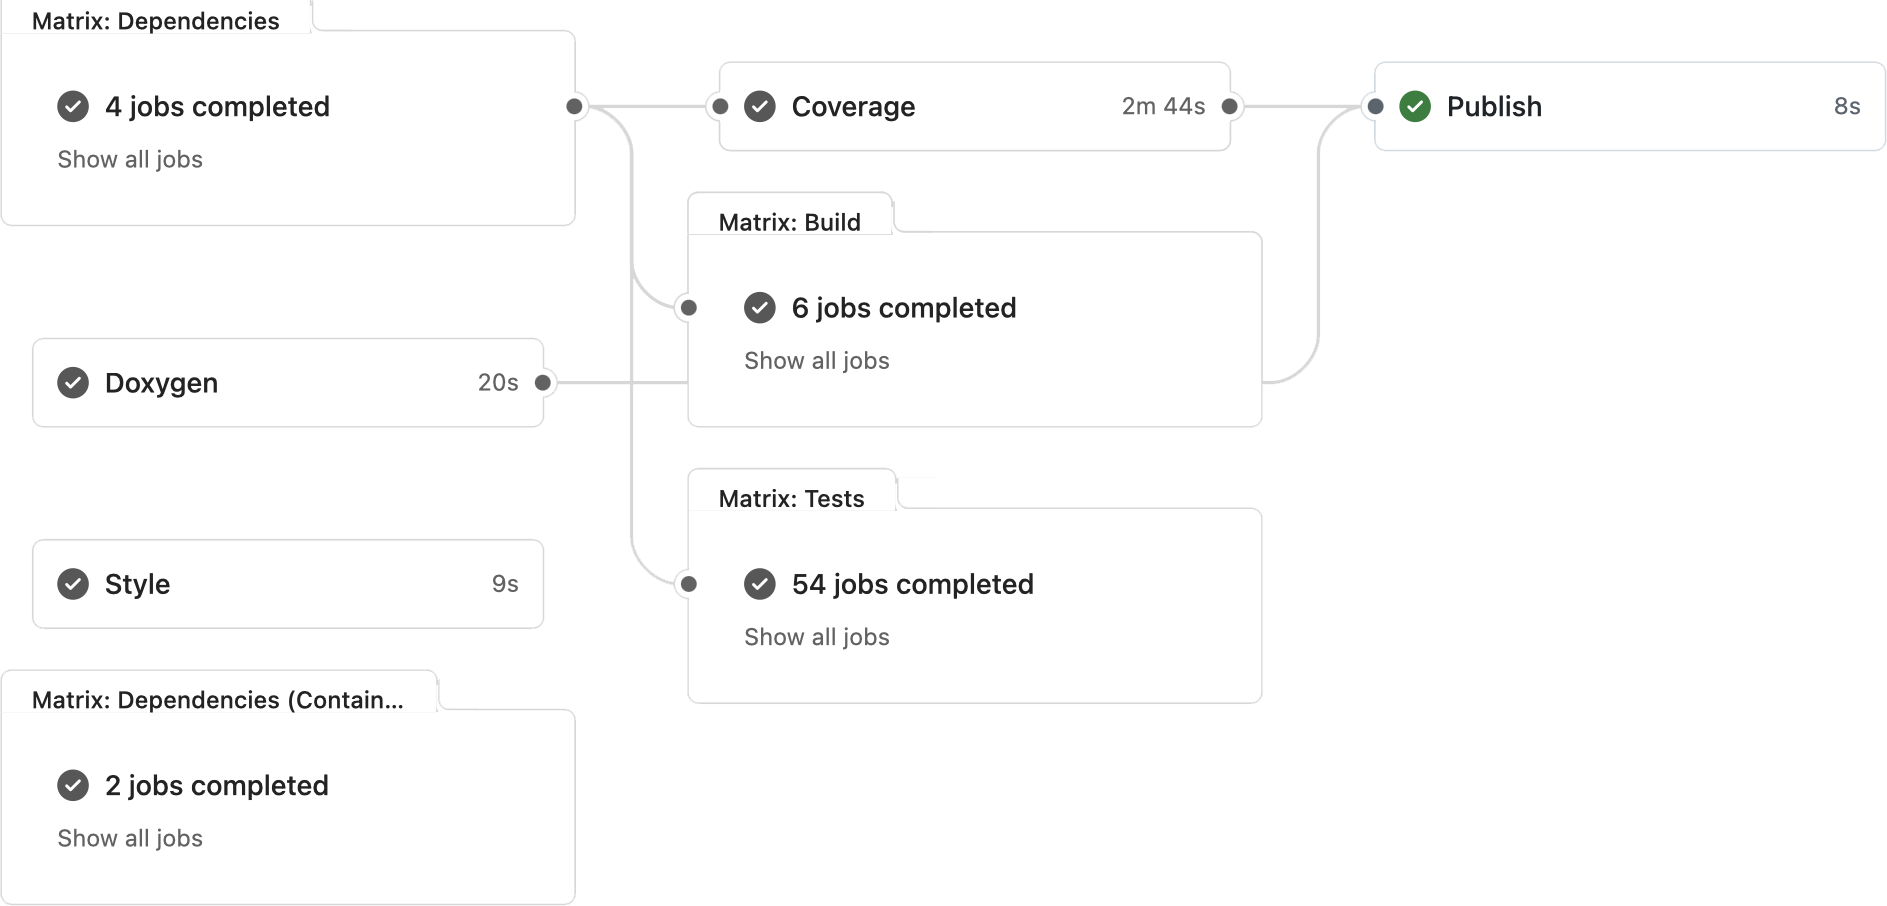
\includegraphics[width=\textwidth]{julea-ci-cd-full.png}
    \caption{CI/CD-Pipeline von Julea. \newline
        Siehe: https://github.com/parcio/julea/actions/runs/8318540808}
\end{figure}

CI/CD, auch CI/CD-Pipeline genannt, ist die Kombination von Contiguous Integration (CI) und Contiguous Deployment/Contiguous Delivery (CD). Eine CI/CD-Pipeline ist eine automatisierte Abfolge von Schritten, welche das Testen, Kompilieren, Bereitstellen und Ausrollen von Artefakten automatisiert. Oftmals sind solche CI/CD-Pipelines direkt teil einer modernen Versiom-Control-System-Plattform wie z. B. GitHub, GitLab, BitBucket, etc. und regieren somit vollautomatisch auf Code-Änderungen.

\subsection{Contiguous Integration (CI)}

Unter Contiguous Integration (CI) versteht man unter anderem das automatisierte testen und/oder kompilieren von Code.  Dieser automatismus dient dazu den Software-Entwickern Zeit zu erspaaren, wodurch sie sich auf das eigentliche entwickeln fokussieren können.

Im gezeigten Beispiel gehören alle bis auf den letzten Schritt "Publish" zur Contiguous Integration (CI).

\begin{figure}[H]
    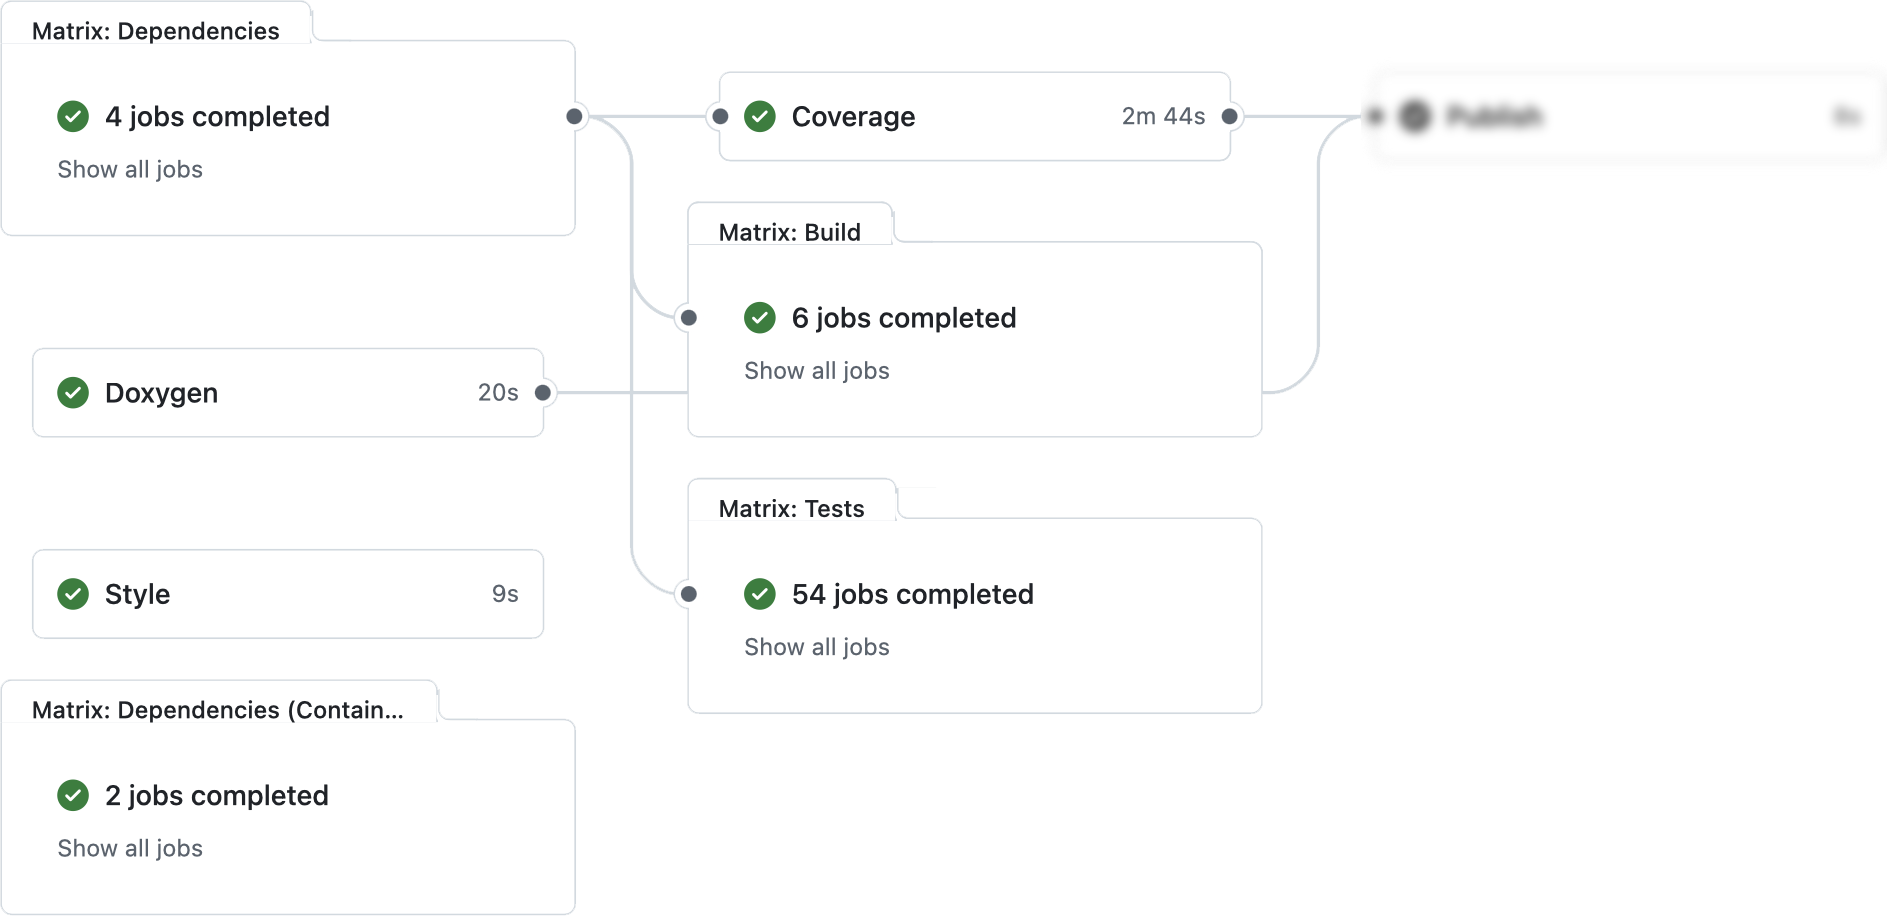
\includegraphics[width=\textwidth]{julea-ci-cd-ci-focus.png}
    \caption{CI/CD-Pipeline von Julea. \newline
        Siehe: https://github.com/parcio/julea/actions/runs/8318540808}
\end{figure}

\subsection{Contiguous Delivery (CD)}

Unter Contiguous Deployment (CD) versteht man das automatisierte bereitstellen von Artefakt. Üblicherweise sind Artefakte Container-Images, ausführbare Dataien, Archive, etc.

Im gezeigten Beispiel gehört nur der letzte Schritt "Publish" zu Contiguous Delivery (CD). In diesem Schritt wird die Dokumentation von Julea automatisch veröffentlicht.

\begin{figure}[H]
    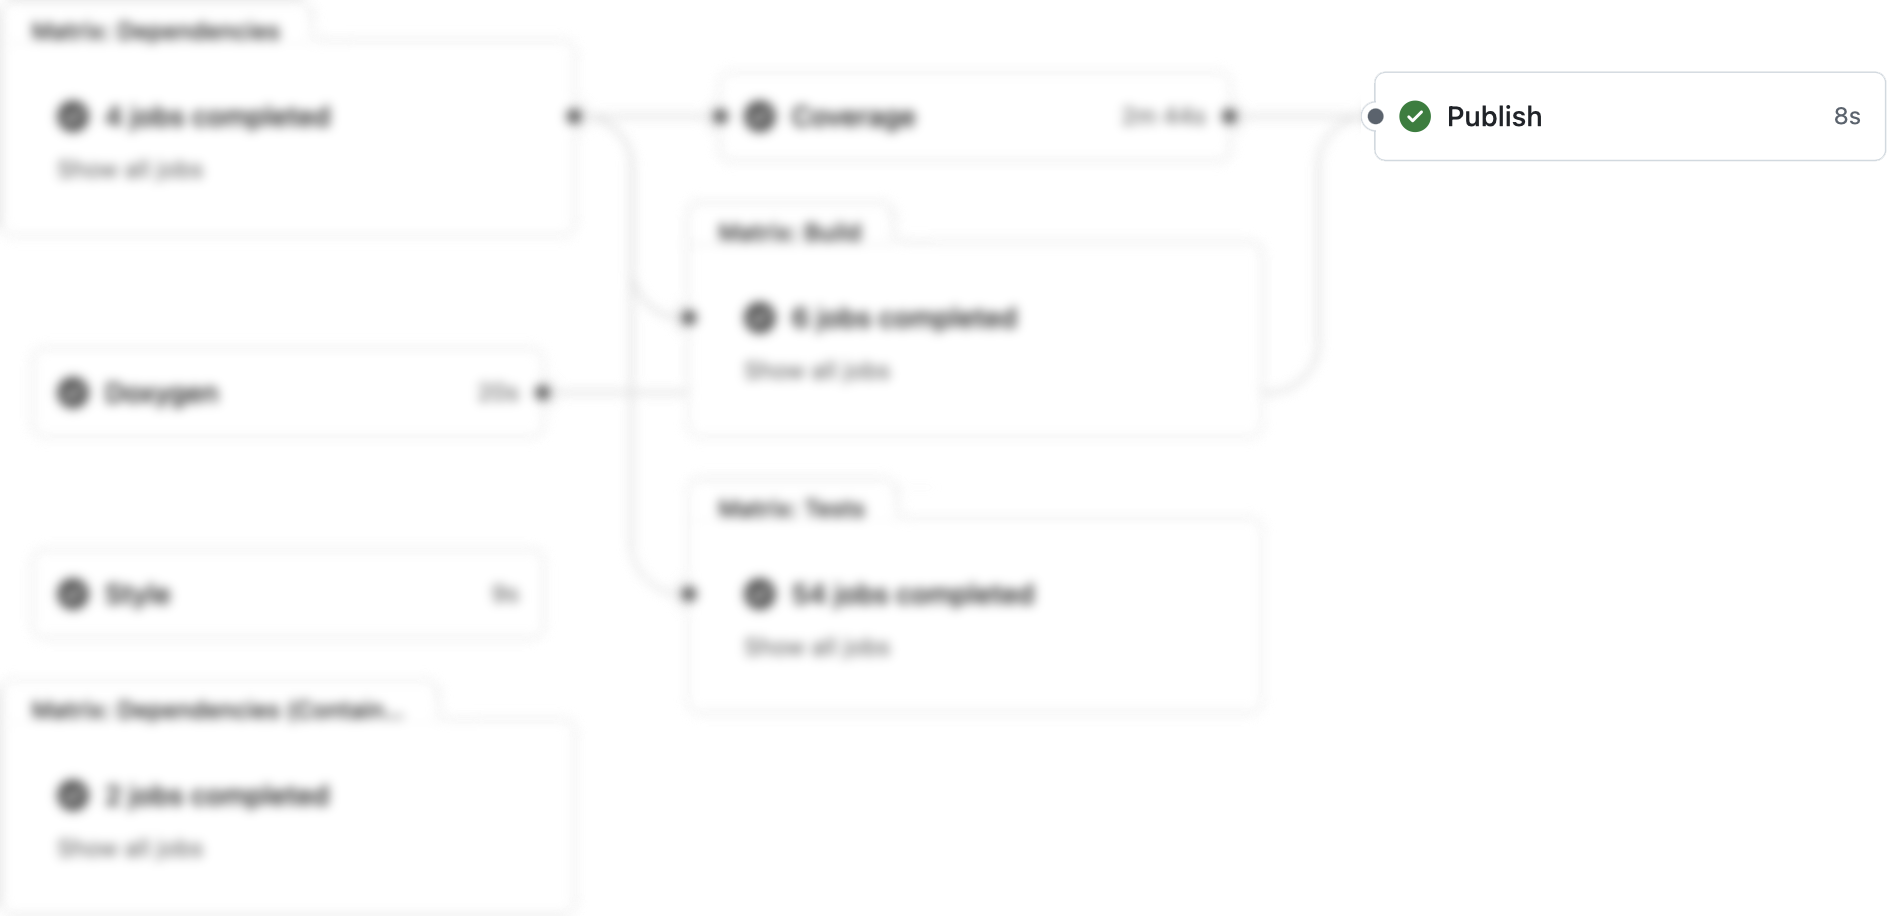
\includegraphics[width=\textwidth]{julea-ci-cd-cd-focus.png}
    \caption{CI/CD-Pipeline von Julea. \newline
        Siehe: https://github.com/parcio/julea/actions/runs/8318540808}
\end{figure}

\subsection{Contiguous Deployment (CD)}

Unter Contiguous Deployment (CD) nimmt das konzept von Contiguous Delivery (CD) auf und rollt das bereitgestellte Artefakt automatisiert aus. In der regel wird das paket auf eine Testumgebung ausgerollt, um sicherzustellen, dass das Artefakt auch tatsächlich stabil lauffähig ist. In der umgebung werden in der Regel automatisierte und/order manuelle Integrationtests durchgeführt. Sollten die tests erfolgreich sein, wird das artefakt sofort oder zu einem release-zeitpunkt auf die Produktivumgebung ausgerollt.

\subsection{GitHub-Actions}

Github-Actions (GHA) ist die GitHub-eigene CI/CD-Pipeline-Lösung. GitHub-Actions ermöglicht es mithilfe einer YML-Datei CI/CD-Pipelines zu definieren. Diese YML-Datei wird im Repository abgelegt und von GitHub-Actions ausgeführt. GitHub-Actions bietet eine Vielzahl von Funktionsbausteinen, welche häufig in CI/CD-Pipelines benötigt werden in einer abstrahierten Form an. Diese bausteine werden entweder von GitHub oder Dritten zur verfügung gestellt. Die bausteine werden in einer isolierten Container-Umgebung ausgeführt, um möglichst reproduzierbare Ergebnisse zu erzielen \cite{githubGitHubActions}.

GitHub-Actions werden als teil dieser Arbeit genutzt, um automatisiert die Julea-Container-Images zu erstellen und zu veröffentlichen.

Diese pipeline baut und veröffentlicht ein Dockerimage, immer wenn ein neuer commit in die "master" Branch gepusht wurde:
\inputminted{yaml}{./code-examples/gha.yml} 

\section{Julea}

In dieser Arbeit wird Julea als Beispiel für eine Applikation verwendet, welche in einem Container-Image bereitgestellt werden soll. Julea ist ein Speicher-Framework, welches mehrere Speicher-Backends wie z. B. Datei-Speicher, MySQL, MongoDB, u. v. m. unterstützt. Julea ist ein Open-Source-Projekt und wird von der Arbeitsgruppe "Parallel Computing and I/O" an der Otto-von-Guericke-Universität Magdeburg entwickelt \cite{kuhnJULEAFlexibleStorage2017}.

Der Quellcode von Julea wird auf GitHub bereitgestellt: \url{https://github.com/parcio/julea}

\section{HPC}

HPC steht für High Performance Computing. HPC-Systeme sind spezielle Computer-Systeme, welche besonders leistungsstark sind. HPC-Systeme werden für berechgnungen mit besonders hohen CPU oder Speicheranforderungen genutzt. Oft werden HPC-Systeme in Forschungseinrichtungen, Universitäten, oder in der Industrie genutzt. HPC-Applikationen sind häufig hochkomplex und greifein auf große mengen von Abhängigkeiten zurück, welche entweder zur Kompilierungszeit, oder zur Laufzeit benötigt werden. Eine hohe anzahl an Abhängigkeiten erschwert das Erstellen von reproduzierbaren Laufzeit-, sowie Kompilierungsergebnissen, da die mögliche kombination von Abhängigkeiten, welche zur Laufzeit und/oder zur Kompilierzeit benötigt werden. 

Die Komplexität von Abhängigkeiten in einer Applikation lässt sich folgendermaßen moddellieren:
\begin{flalign*}
    &\text{Sei } D_a = (x_0,\dots, x_n), x_i \in \mathbb{N} \\&
    \text{und } x_i \text{ die Anzahl der akzeptierten Variationen der }i\text{-ten Abhängigkeit der Applikation } a&
\end{flalign*}
Dann ist die Anzahl der unterschiedlichen Umgebunden, in der die Applikation $a$ funktionieren sollte: 
\begin{align*}
   \prod_{i=0}^{|D_a|} x_i
\end{align*}

Angenommen, es gibt eine Applikation $b$, welche 3 Abhängigkeiten mit jeweils 3 akzeptierten varianten hat ($D_b = (3, 3, 3)$), dann ist: 
\begin{align*}
    \prod_{i=0}^{|D_b|} x_i &= \prod_{i=0}^{3} x_i\\
    &= 3 \cdot 3 \cdot 3 \\
    &= 27
\end{align*}

Seien:
\begin{align*}
    f(n) &= (x_i)_{i=0}^{n}, \text{wobei } n \in \mathbb{N} \text{ und } x_i = 3 \\
    g(n) &= \prod_{i=0}^{|f(n)|} f(n)
\end{align*}

Dann stellt $g(n)$ die Anzahl der unterschiedlichen Umgebungen für $n$ Abhängigkeiten mit jeweils 3 akzeptierten Variationen je Abhängigkeit dar:

\begin{tikzpicture}
    \begin{axis}[
        axis lines = left,
        xlabel = \(n\),
        ylabel = {\(g(n)\)},
    ]
    %Below the red parabola is defined
    \addplot [
        domain=0:6,
        samples=100, 
        color=red,
    ]
    {3^x};
    \addlegendentry{\(\prod_{i=0}^{|f(n)|} f(n)\)}
    
    \end{axis}
\end{tikzpicture}

Es wird ersichtlich, dass die Anzahl der unterschiedlichen Umgebungen exponentiell mit der Anzahl der akzeptierten Variationen wächst. 

Dies bedeutet, dass Applikationen, welche sehr viele Abhängigkeiten haben, und diese Abhängigkeiten selbst mehrere variationen (Versionen, Kompilierung-Flags, etc.) haben ist es unmöglich jede mögliche Umgebung zu testen. Es ist in diesen Fall einfacher eine möglich konsistente Umgebung zu schaffen. Übliche mechanismen eine solche konsistente Umgebung zu schaffen ist Virtualisierung oder das Eliminieren von mehreren akzeptierten Abhängigkeitsvariationen durch Version-Pinning. Hierbei ist allerdings zu beachten, dass Version-Pinning nicht indirekte Abhängigkeiten konsistent hält. Dies ist bei der Virtualisierung anders. Die Hardwarevirtualisierung stellt sicher, dass alles bis zur Hardware-Ebende konsistent gehalten werden kann, dies kommt üblicherweise mit performance-einbußen einher und einem großen Paket, welches ausgerollt werden müsste. Hier bietet die Containervisualisierung einen mittelweg, indem es alles bis zum Betriebssystem konsistent hält und somit kaum bis garkein Performanceoverhead, sowie eine – im Vergleich zur Hardwarevirtualisierung – kleinere Paketgröße.
